\subsection{Image-processing outputs}
The integrated pipeline retains seven connected components after cleanup and
splits wide regions into ten ordered boxes. Figure labels are manual reference
annotations, not predicted labels. The group must verify crop quality and
provide its own interpretation of the comparisons below.
\begin{figure}[htbp]\centering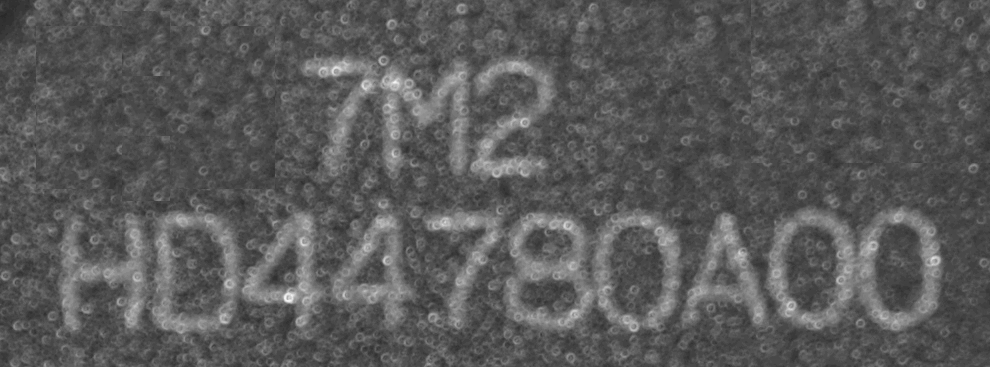
\includegraphics[width=\linewidth,height=0.40\textheight,keepaspectratio]{../results/figures/01_original.png}\caption{Original chip image.}\end{figure}
\begin{figure}[htbp]\centering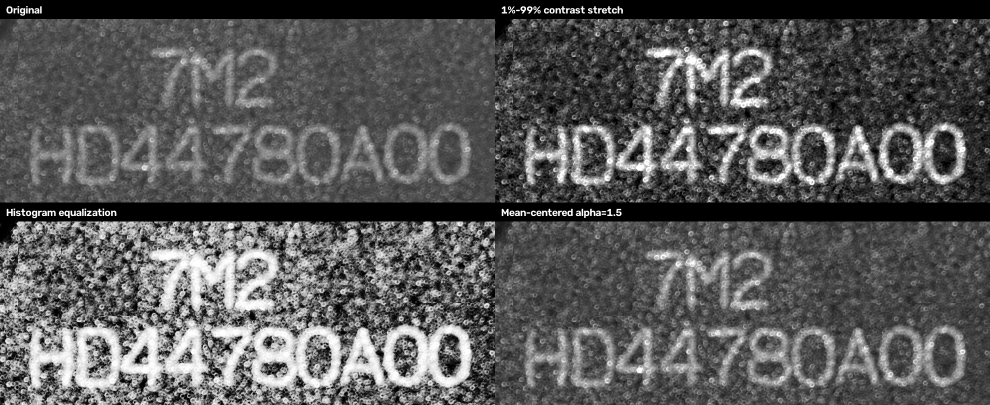
\includegraphics[width=\linewidth,height=0.40\textheight,keepaspectratio]{../results/figures/task1_contrast_comparison.png}\caption{Task 1 enhancement comparison.}\end{figure}
\begin{figure}[htbp]\centering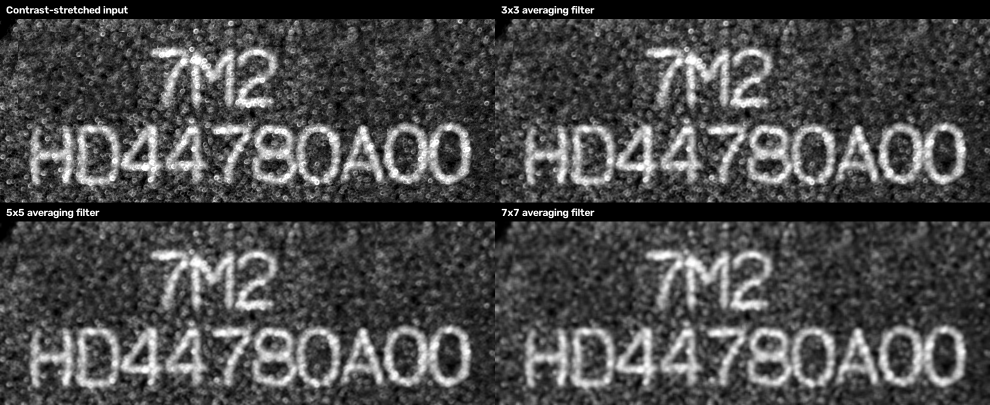
\includegraphics[width=\linewidth,height=0.40\textheight,keepaspectratio]{../results/figures/task2_mean_filter_comparison.png}\caption{Task 2 averaging filter comparison.}\end{figure}
\begin{figure}[htbp]\centering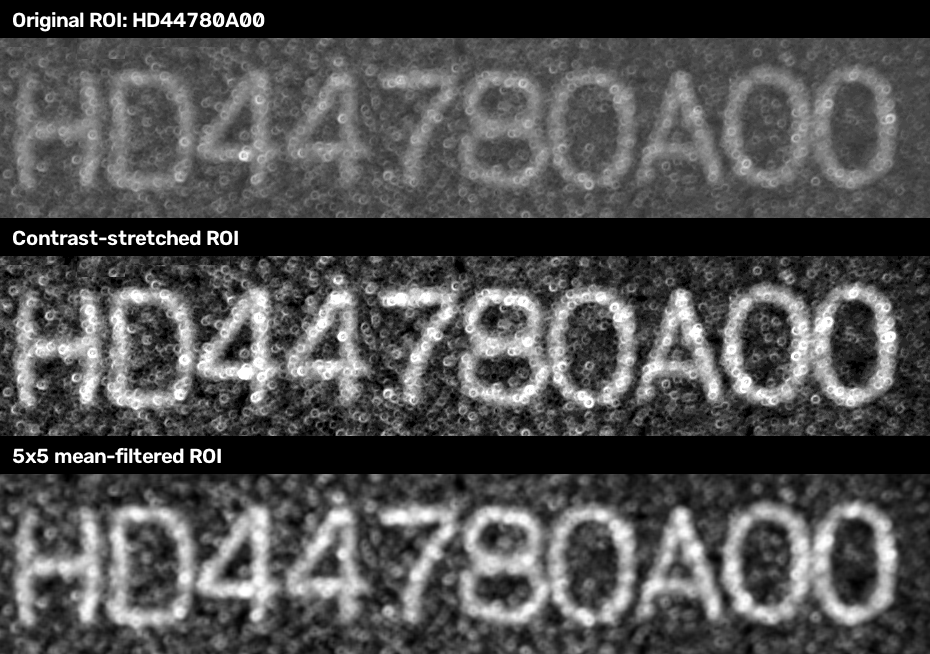
\includegraphics[width=\linewidth,height=0.40\textheight,keepaspectratio]{../results/figures/task3_roi_comparison.png}\caption{Task 3 ROI comparison.}\end{figure}
\begin{figure}[htbp]\centering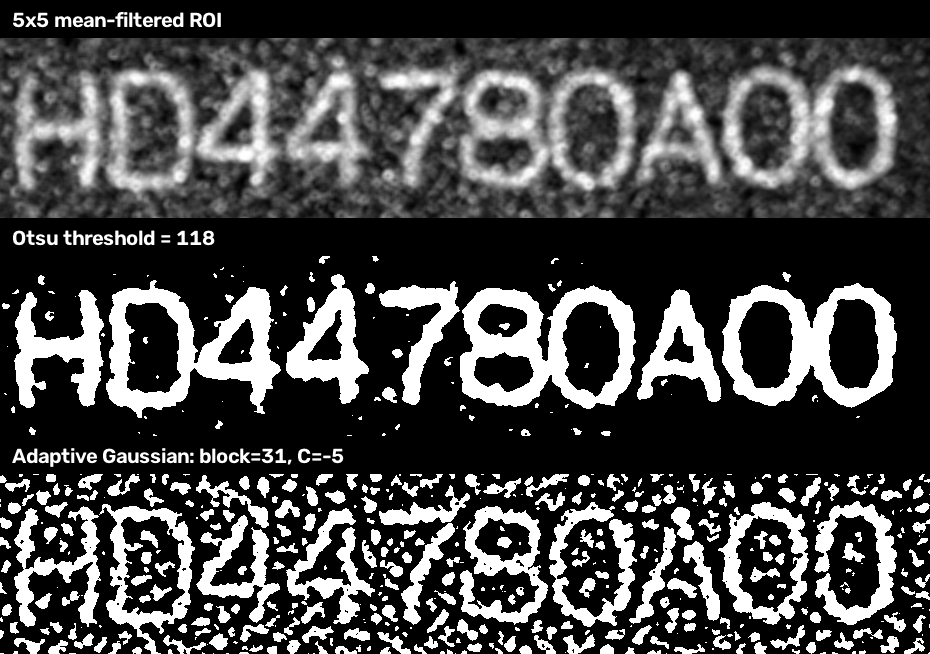
\includegraphics[width=\linewidth,height=0.40\textheight,keepaspectratio]{../results/figures/task4_binarization_comparison.png}\caption{Task 4 thresholding comparison.}\end{figure}
\begin{figure}[htbp]\centering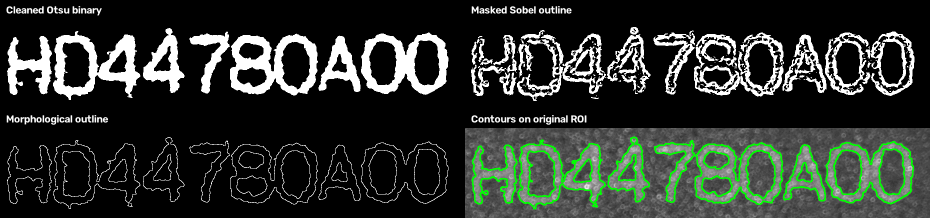
\includegraphics[width=\linewidth,height=0.40\textheight,keepaspectratio]{../results/figures/task5_outline_comparison.png}\caption{Task 5 outline comparison.}\end{figure}
\begin{figure}[htbp]\centering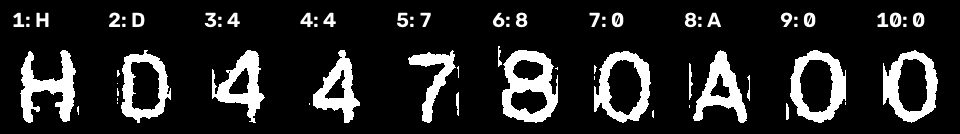
\includegraphics[width=\linewidth,height=0.40\textheight,keepaspectratio]{../results/figures/task6_character_strip.png}\caption{Task 6 crops with manual reference labels.}\end{figure}
\begin{figure}[htbp]\centering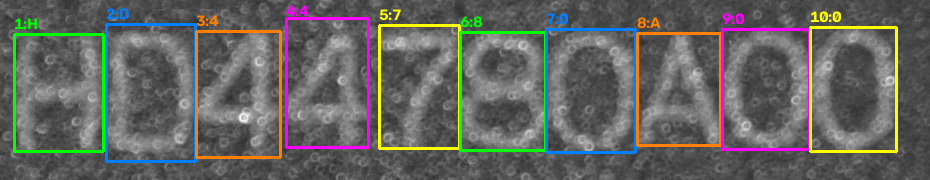
\includegraphics[width=\linewidth,height=0.40\textheight,keepaspectratio]{../results/figures/17_labeled_characters.png}\caption{Task 6 ordered boxes with manual reference annotations.}\end{figure}
\clearpage\subsection{Measured classification outputs}\begin{center}\begin{tabular}{lrrl}\toprule
Model & Test accuracy (\%) & Training (s) & Chip prediction \\ \midrule
baseline & 98.93 & 30.31 & HD4A780A00 \\
yjn & 92.69 & 33.69 & 8848888A88 \\
hog-svm & 98.37 & 0.63 & AAAAAAAAAA \\
\bottomrule\end{tabular}\end{center}
Chip inference inverts binary crops to dark glyphs on a white background, matching the training images. Baseline still misclassifies one target character; YJN and SVM fail on most chip crops despite high dataset accuracy. These are recorded failures, not successful end-to-end recognition. These values are automated measurements; interpretation and final conclusions must be supplied by the group. Training times exclude preprocessing and feature extraction and are not total pipeline costs.
\subsection{Per-class evaluation}
\paragraph{baseline}\begin{center}\begin{tabular}{lrrrr}\toprule Class & Precision & Recall & F1 & Support \\ \midrule
0 & 1.000 & 0.988 & 0.994 & 254 \\
4 & 1.000 & 0.984 & 0.992 & 254 \\
7 & 0.992 & 1.000 & 0.996 & 254 \\
8 & 1.000 & 0.988 & 0.994 & 254 \\
A & 0.977 & 0.992 & 0.984 & 254 \\
D & 0.981 & 0.992 & 0.986 & 254 \\
H & 0.976 & 0.980 & 0.978 & 254 \\
\bottomrule\end{tabular}\end{center}
\noindent Confusion matrix (rows: true, columns: predicted; order 0,4,7,8,A,D,H):
\begin{center}\begin{tabular}{rrrrrrr}
251 & 0 & 0 & 0 & 0 & 2 & 1 \\
0 & 250 & 0 & 0 & 2 & 0 & 2 \\
0 & 0 & 254 & 0 & 0 & 0 & 0 \\
0 & 0 & 0 & 251 & 1 & 2 & 0 \\
0 & 0 & 0 & 0 & 252 & 0 & 2 \\
0 & 0 & 0 & 0 & 1 & 252 & 1 \\
0 & 0 & 2 & 0 & 2 & 1 & 249 \\
\end{tabular}\end{center}
\paragraph{yjn}\begin{center}\begin{tabular}{lrrrr}\toprule Class & Precision & Recall & F1 & Support \\ \midrule
0 & 0.975 & 0.937 & 0.956 & 254 \\
4 & 0.907 & 0.996 & 0.949 & 254 \\
7 & 0.984 & 0.996 & 0.990 & 254 \\
8 & 0.873 & 1.000 & 0.932 & 254 \\
A & 0.814 & 0.984 & 0.891 & 254 \\
D & 1.000 & 0.874 & 0.933 & 254 \\
H & 1.000 & 0.701 & 0.824 & 254 \\
\bottomrule\end{tabular}\end{center}
\noindent Confusion matrix (rows: true, columns: predicted; order 0,4,7,8,A,D,H):
\begin{center}\begin{tabular}{rrrrrrr}
238 & 1 & 0 & 11 & 4 & 0 & 0 \\
0 & 253 & 1 & 0 & 0 & 0 & 0 \\
0 & 1 & 253 & 0 & 0 & 0 & 0 \\
0 & 0 & 0 & 254 & 0 & 0 & 0 \\
0 & 2 & 0 & 2 & 250 & 0 & 0 \\
6 & 1 & 1 & 15 & 9 & 222 & 0 \\
0 & 21 & 2 & 9 & 44 & 0 & 178 \\
\end{tabular}\end{center}
\paragraph{hog-svm}\begin{center}\begin{tabular}{lrrrr}\toprule Class & Precision & Recall & F1 & Support \\ \midrule
0 & 0.992 & 0.988 & 0.990 & 254 \\
4 & 1.000 & 0.996 & 0.998 & 254 \\
7 & 0.996 & 0.988 & 0.992 & 254 \\
8 & 0.992 & 0.976 & 0.984 & 254 \\
A & 0.937 & 0.996 & 0.966 & 254 \\
D & 0.988 & 0.980 & 0.984 & 254 \\
H & 0.984 & 0.961 & 0.972 & 254 \\
\bottomrule\end{tabular}\end{center}
\noindent Confusion matrix (rows: true, columns: predicted; order 0,4,7,8,A,D,H):
\begin{center}\begin{tabular}{rrrrrrr}
251 & 0 & 0 & 2 & 1 & 0 & 0 \\
0 & 253 & 0 & 0 & 0 & 0 & 1 \\
0 & 0 & 251 & 0 & 1 & 0 & 2 \\
1 & 0 & 0 & 248 & 4 & 1 & 0 \\
1 & 0 & 0 & 0 & 253 & 0 & 0 \\
0 & 0 & 0 & 0 & 4 & 249 & 1 \\
0 & 0 & 1 & 0 & 7 & 2 & 244 \\
\end{tabular}\end{center}
